\subsection{Обучение моделей на датасете MultiAtis++}
В своей работе мы обучаем языковые модели решать задачу задачи одновременного детектирования намерений пользователя и заполнения слотов для диалоговых помощников, направленных на выполнение конкретной задачи.
Эта задача заключается в классификации предложений и всех слов в предложении.

\subsubsection{Датасет}
В качестве датасета в своей работе мы выбрали датасет MultiAtis++~\cite{Xu2020EndtoEndSA}.
В этом датасете представлены семь языков из трёх языковых семей —
Индо-Европейская (английский, немецкий, французский, испанский, португальский), Японо-рюкюская (японский) и Сино-тибетская (китайский).
Датасет является параллельным корпусом для задачи классификации интентов и разметки слотов - в 2020 году он был переведён с английского языка на остальные шесть.
В обучающей выборке содержится 4978 предложений для каждого языка, в тестовой 893 предложения для каждого языка.

\begin{table}[H]
    \resizebox{\textwidth}{!}{
        \begin{tabular}{|>{\bfseries}c|ccccccc|}
            \hline
            Intent & \multicolumn{7}{c|}{ atis\_flight } \\ \hline
            Utterance en   & show  & me  & flights & from & montreal             & to   & orlando            \\ \hline
            Slot labels en & O     & O   & O       & O    & B-fromloc.city\_name & O    & B-toloc.city\_name \\ \hline
            Utterance de   & Zeige & mir & Flüge   & von  & Montreal             & nach & Orlando            \\ \hline
            Slot labels de & O     & O   & O       & O    & B-fromloc.city\_name & O    & B-toloc.city\_name \\ \hline
        \end{tabular}
    }\caption{Пример объекта из датасета MultiAtis++. На примере представлен объект на английском и немецком языке.}\label{tab:table}
\end{table}

\parКаждый объект в датасете состоит из предложения, меток слов в BIO формате и интента (Таблица~\eqref{tab:table}).
Перед началом работы с датасетом мы произвели предварительную очистку —
убрали из обучающей и тестовой выборок объекты, для которых на любом из семи языков количество слов и количество слотов не совпадали.
Таким образом, в обучающей выборке осталось 4884 объекта для каждого языка, в тестовой выборке 755 объектов для каждого языка.
Для составления списка используемых слотов и интентов использовалась обучающая выборка на английском языке.
Мы использовали 121 различную метку слотов и 23 различных метки интентов.

\subsubsection{Архитектура модели}
В своей работе мы решаем задачу одновременной классификации интентов и разметки слотов в предложении с помощью одной модели.
Модель имеет два выхода, первый предсказывает интенты, второй предсказывает метки слов.
В качестве рассматриваемых архитектур были выбраны модели m-BERT~\cite{devlin-etal-2019-bert} и XLM-RoBERTa~\cite{Conneau2020UnsupervisedCR}.
Обе эти модели являются одними из самых сильных мультиязычных моделей на текущий момент.
Каждая из них предобучена на более чем ста языках.
\parОбозначим количество блоков Трансформера за L, размер скрытых представлений за H и количество голов с внутренним вниманием за A\@.
Тогда в используемой нами модели m-BERT L = 12, H = 768, A = 12, а суммарное количество параметров 110 миллионов.
В используемой нами модели XLM-RoBERTa L = 12, H = 768, A = 12, а суммарное количество параметров 270 миллионов.

\subsubsection{Обучение}\label{subsubsec:model_name}
В своей работе мы будем сравнивать модели, обученные на всей обучающей выборке и только на части обучающей выборки на английском языке.
Таким образом мы сможем проверить насколько устойчивы к нашим атакам модели с разными вариантами обучения.
\parВведем краткие обозначения для удобства — модели XLM-RoBERTa будут обозначаться как <<xlm-r>>, модели m-BERT будут обозначаться как <<m-bert>>.
Если модель обучалась только на английской подвыборке, то мы будем добавлять в её название суффикс <<en>>.
\parКаждая из моделей обучалась с одинаковыми гиперпараметрами - 10 эпох на обучающей выборке с длиной шага обучения $10^{-5}$ и размером батча в 64 объекта.
В качестве функции ошибки использовалась кросс-энтропия:
\begin{equation}
    \mathcal{L} = -\dfrac{1}{n}\sum\limits_{i = 1}^{n}\left[ y\log\left(\hat{y}\right) \right]\label{eq:equation4}
\end{equation}
\parВ своей работе мы будем использовать следующие метрики качества:
\begin{itemize}
    \item Доля предложений, в которых правильно классифицирован интент:
    \begin{equation}
        \textbf{Intent accuracy} = \# \text{sentences} \left[ \left(I_{pred} = I_{true} \right) \right]\label{eq:equation}
    \end{equation}
    \item F1 мера для меток слотов (используется микро-усреднение по всем классам):
    \begin{equation}
        \textbf{Slots F1 score} = 2 \cdot \dfrac{\text{precision} \cdot \text{recall}}{\text{precision} + \text{recall}}\label{eq:equation2}
    \end{equation}
    \item Доля предложений, в которых правильно классифицирован интент и верно классифицированы все слоты:
    \begin{equation}
        \textbf{Semantic accuracy} = \# \text{sentences} \left[ \left(I_{pred} = I_{true} \right) \land \left(S_{pred} = S_{true} \right)\right]\label{eq:equation3}
    \end{equation}
\end{itemize}

\newpage

\subsection{Адверсариальные атаки}
В своей работе мы предлагаем два варианта gray-box адверсариальных атак — во время выполнения атаки мы имеем доступ к ошибке модели.
Мы стремимся создать атаку такого рода, чтобы результирующая адверсариальная пертурбация предложения была как можно ближе к реалистичным предложениям со смешением кодов.
Оценка качества на таких адверсариальных атаках может выступать в роли оценки снизу на качество соответствующих моделей в аналогичных задачах при наличии реального смешения кодов во входных данных.
\parМы фокусируемся в основном на лексической части смешения кодов — когда некоторые слова заменяются за их аналоги из других языков.
Во время атаки мы заменяем часть токенов в предложении на их эквиваленты из атакующих языков, метод определения эквивалентов зависит от типа атаки.
Так как большинство людей, которые могут использовать смешение кодов в своей речи, билингвы, то в основном смешение кодов происходит между парой языков~\cite{bilinguals}.
Таким образом, в своей работе мы предлагаем анализировать атаки состоящие во встраивании одного языка в другой.

\subsubsection{Общий вид атаки}
Общий принцип атаки одинаковый для обоих предлагаемых вариантов.
Разница между методами заключается в способе генерации кандидатов на замену токену на $i-$ой позиции.
В своей работе мы предлагаем следующий вид атаки — пусть мы имеем целевую модель, пару пример-метка и встраиваемый язык (Алгоритм~\eqref{alg:algorithm}).
Тогда мы перебираем токены в предложении в случайном порядке и стремимся заменить токен на его эквивалент из встраиваемого языка.
Если это приведёт к увеличению ошибки модели, то мы заменяем токен на предложенного кандидата.

\begin{algorithm}
    \caption{Общая схема адверсариальной атаки}
    \begin{algorithmic}
        \Require{Пара пример-метка x, y; целевая модель $\mathcal{M}$; встраиваемый язык $\mathbb{L}$}
        \Ensure{Адверсариальный пример x'} \\
        $\mathcal{L}_{x}$ = GetLoss($\mathcal{M}$, x, y)
        \For{i in permutation(len(x))}
            \\
            \ind Candidates = GetCandidates($\mathcal{M}$, x, y, token\_id = i) \\
            \ind Losses = GetLoss($\mathcal{M}$, Candidates)
            \ind\If{Candidates and max(Losses) > $\mathcal{L}_{x}$}
                    \\
                    \ind\ind$\mathcal{L}_{x}$ = max(Losses) \\
                    \ind\ind x, y = Candidates[argmax(Losses)]
            \EndIf
        \EndFor \\
        \ind\Return x
    \end{algorithmic}\label{alg:algorithm}
\end{algorithm}

\subsubsection{Word-level атака}
Первый предлагаемый нами вариант атаки заключается в генерации эквивалентов из других языков с помощью перевода токенов на соответствующие языки (Алгоритм~\eqref{alg:algorithm1}).
Атакуя таким образом, мы строим грубую оценку снизу, так как при атаке мы не учитываем контекста предложений и не учитываем многозначность слов.
Этот вариант схож с атакой PolyGloss~\cite{Tan2021CodeMixingOS}.
Примеры атаки на тестовую выборку для модели XLM-RoBERTa можно найти в таблицах ~\eqref{tab:table18},\eqref{tab:table19} и~\eqref{tab:table20}.
\parДля перевода слов на другие языки мы используем модель машинного перевода M2M 100 от компании Facebook~\cite{Fan2020BeyondEM}.
Она содержит 418 миллионов параметров.
\par Псевдокод функции ExtendSlotLabels можно найти в приложении (Алгоритм~\eqref{alg:algorithm3}).

\begin{algorithm}
    \caption{Word-level атака}
    \begin{algorithmic}
        \Require{Словарь переводов с исходного на встраиваемый язык $\mathbb{T}$}
        \Function{GetCandidates}{$\mathcal{M}$, x, y, token\_id}
            \ind\If{x[token\_id] in $\mathbb{T}[\mathbb{L}]$}
                    \\
                    \ind\ind tokens = $\mathbb{T}[\mathbb{L}]$[x[token\_id]]\\
                    \ind\ind x[token\_id] = tokens\\
                    \ind\ind y[token\_id] = ExtendSlotLabels(y[token\_id], len(tokens))
            \EndIf \\
            \ind\Return x, y
        \EndFunction
    \end{algorithmic}\label{alg:algorithm1}
\end{algorithm}

\begin{table}[H]
	\resizebox{\textwidth}{!}{
		\begin{tabular}{|>{\bfseries}l|ccccccccc|}
			\hline
			Utterance en &what & are & the & flights & from & tacoma & to & san & jose \\ \hline
			Utterance adv &what & are & El & vuelos & from & tacoma & to & san & jose \\ \hline
		\end{tabular}
	}\caption{Пример 1 атаки модели XLM-RoBERTa (xlm-r) word-level атакой.}\label{tab:table18}
\end{table}
\begin{table}[H]
	\resizebox{\textwidth}{!}{
		\begin{tabular}{|>{\bfseries}l|ccccccccccc|}
			\hline
			Utterance en &i & would & like & flight & information & from & phoenix & to & denver &   &   \\ \hline
			Utterance adv &y & would & como & flight & Información & from & El & Phoenix & para & El & Denver \\ \hline
		\end{tabular}
	}\caption{Пример 2 атаки модели XLM-RoBERTa (xlm-r) word-level атакой.}\label{tab:table19}
\end{table}
\begin{table}[H]
	\resizebox{\textwidth}{!}{
		\begin{tabular}{|>{\bfseries}l|ccccccccc|}
			\hline
			Utterance en &what & are & the & flights & from & las & vegas & to & ontario \\ \hline
			Utterance adv &what & sind & Die & flights & from & las & VEGAS & to & ontario \\ \hline
		\end{tabular}
	}\caption{Пример 3 атаки модели XLM-RoBERTa (xlm-r) word-level атакой.}\label{tab:table20}
\end{table}


\subsubsection{Phrase-level атака}
Второй предлагаемый нами вариант атаки заключается в генерации эквивалентов из других языков с помощью построения выравниваний между предложениями на разных языках (Алгоритм~\eqref{alg:algorithm2}).
Одно предложение является переводом другого, для перевода можно использовать ту же модель машинного перевода~\cite{Fan2020BeyondEM}, однако мы пользуемся тем, что у нас уже параллельный корпус.
Кандидаты для каждого токена определяются как токены из предложения на встраиваемом языке, в которые был выровнен токен.
Этот вариант атаки схож с атакой Bumblebee~\cite{Tan2021CodeMixingOS}.
Примеры атаки на тестовую выборку для модели XLM-RoBERTa можно найти в таблицах ~\eqref{tab:table21},\eqref{tab:table22} и~\eqref{tab:table23}.
\parДля построения выравниваний мы используем модель awesome-align на основе m-BERT~\cite{Dou2021WordAB}.

\begin{algorithm}
    \caption{Phrase-level атака}
    \begin{algorithmic}
        \Require{Выравнивание предложения на исходном языке к предложению на целевом языке $\mathbb{A}$}
        \Function{GetCandidates}{$\mathcal{M}$, x, y, token\_id}
            \If{x[token\_id] in $\mathbb{A}[\mathbb{L}]$}
                \\
                \ind\ind tokens = $\mathbb{A}[\mathbb{L}]$[x[token\_id]]\\
                \ind\ind x[token\_id] = tokens\\
                \ind\ind y[token\_id] = ExtendSlotLabels(y[token\_id], len(tokens))
            \EndIf \\
            \ind\Return x, y
        \EndFunction
    \end{algorithmic}\label{alg:algorithm2}
\end{algorithm}

\begin{table}[H]
	\resizebox{\textwidth}{!}{
		\begin{tabular}{|>{\bfseries}l|ccccccccc|}
			\hline
			Utterance en &please & find & flights & available & from & kansas & city & to & newark \\ \hline
			Utterance adv &encontre & find & flights & disponíveis & from & kansas & City & para & Newark \\ \hline
		\end{tabular}
	}\caption{Пример 1 атаки модели XLM-RoBERTa (xlm-r) phrase-level атакой.}\label{tab:table21}
\end{table}
\begin{table}[H]
	\resizebox{\textwidth}{!}{
		\begin{tabular}{|>{\bfseries}l|ccccccccc|}
			\hline
			Utterance en &what & are & the & flights & from & tacoma & to & san & jose \\ \hline
			Utterance adv &cuáles & are & the & flights & from & tacoma & a & san & jose \\ \hline
		\end{tabular}
	}\caption{Пример 2 атаки модели XLM-RoBERTa (xlm-r) phrase-level атакой.}\label{tab:table22}
\end{table}
\begin{table}[H]
	\resizebox{\textwidth}{!}{
		\begin{tabular}{|>{\bfseries}l|ccccccccc|}
			\hline
			Utterance en &show & flights & saturday & evening & from & st. & louis & to & burbank \\ \hline
			Utterance adv &show & flights & sábado & evening & from & St. & Louis & para & Burbank \\ \hline
		\end{tabular}
	}\caption{Пример 3 атаки модели XLM-RoBERTa (xlm-r) phrase-level атакой.}\label{tab:table23}
\end{table}


\newpage

\subsection{Метод адверсариального предобучения для защиты от адверсариальных атак}
В своей работе мы предлагаем метод защиты от предложенных выше адверсариальных атак.
Гипотеза заключается в том, что данный метод позволит увеличить качество не только на адверсариальных пертурбациях, но и на реальных данных со смешением кодов.
\parПредлагаемый нами метод адверсариального предобучения состоит из нескольких шагов:
\begin{enumerate}
    \item Генерация выборки для задачи маскированного моделирования языка.
    \item Дообучение тела мультиязычной модели на сгенерированной выборке в режиме предсказания маскированных токенов.
    \item Загрузка дообученного тела модели перед началом обучения для задачи одновременного заполнения слотов и классификации интентов.
\end{enumerate}

\begin{algorithm}
    \caption{Генерация адверсариальной выборки}
    \begin{algorithmic}
        \Require{Обучающая выборка датасета $X$, набор встраиваемых языков $\mathbb{L}_1, \dots \mathbb{L}_n$}
        \Ensure{Адверсариальная выборка $X'$} \\
        X' = [~]
        \For{$\mathbb{L}$ in $\mathbb{L}_1, \dots \mathbb{L}_n$}
            \For{x in X}
                \For{i in permutation(len(x))}
                    \\
                    \ind\ind\ind Candidates = GetCandidates($\mathcal{M}$, x, y, token\_id = i)
                    \ind\If{Candidates and $\unif$(0, 1) > 0.5}
                            \\
                            \ind\ind\ind\ind x, \_ = random.choice(Candidates)
                    \EndIf
                \EndFor \\
                \ind\ind X`.append(x)
            \EndFor
        \EndFor \\
        \Return X'
    \end{algorithmic}\label{alg:algorithm4}
\end{algorithm}

\subsubsection{Генерация адверсариальной выборки}
Для генерации выборки используется адаптация алгоритма phrase-level адверсариальной атаки (Алгоритм~\eqref{alg:algorithm4}).
Разница заключается в том, что токены заменяются на их эквиваленты с некоторой вероятностью.
Таким образом, для генерации выборки не требуется обученная модель.
\parВыборка является конкатенацией сгенерированных выборок для всех языков представленных в датасете кроме английского .
Каждая из подвыборок генерируется встраиванием целевого языка в обучающую выборку датасета MultiAtis++ на английском языке.
Псевдокод функции GetCandidates представлен в секции про атаки (Алгоритм~\eqref{alg:algorithm2}).
\parПосле генерации у нас получается 6 подвыборок по 4884 предложения в каждой.
Итоговая выборка состоит из 29304 предложений, мы делим эту выборку в отношении 9 к 1 на обучающую и тестовую.
Примеры объектов из адверсариальной выборки -~\eqref{tab:table40},~\eqref{tab:table41} и~\eqref{tab:table42}.

\begin{table}[H]
	\resizebox{\textwidth}{!}{
		\begin{tabular}{|>{\bfseries}l|ccccccccc|}
			\hline
			Utterance en &what & flights & from & las & vegas & to & phoenix & on & saturday \\ \hline
			Utterance adv &Quels & vols & de & las & Vegas & à & phoenix & on & saturday \\ \hline
		\end{tabular}
	}\caption{Пример 1 из адверсариальной выборки.}\label{tab:table40}
\end{table}
\begin{table}[H]
	\resizebox{\textwidth}{!}{
		\begin{tabular}{|>{\bfseries}l|ccccccccc|}
			\hline
			Utterance en &show & me & the & flights & from & denver & to & westchester & county \\ \hline
			Utterance adv &Mostre & me & os & flights & de & denver & to & Westchester & County \\ \hline
		\end{tabular}
	}\caption{Пример 2 из адверсариальной выборки.}\label{tab:table41}
\end{table}
\begin{table}[H]
	\resizebox{\textwidth}{!}{
		\begin{tabular}{|>{\bfseries}l|ccccccccc|}
			\hline
			Utterance en &show & me & all & flights & from & san & francisco & to & atlanta \\ \hline
			Utterance adv &show & me & all & flights & de & São & Francisco & to & Atlanta \\ \hline
		\end{tabular}
	}\caption{Пример 3 из адверсариальной выборки.}\label{tab:table42}
\end{table}


\subsubsection{Дообучение тела модели}
После генерации адверсариальной выборки мы дообучаем предобученную мультиязычную модель на этой выборке.
Модель обучается в режиме задачи маскированного моделирования языка.
\parДля обучения модели для такой задачи мы отбираем 15\% токенов и предсказываем их с помощью модели.
80\% отобранных токенов заменяются на токен маски, 10\% заменяются на случайные слова из словаря, остальные 10\% остаются неизменными~\cite{devlin-etal-2019-bert}.
Мы дообучаем обе мультиязычные модели m-BERT и XLM-RoBERTa с одинаковыми гиперпараметрами - 10 эпох с размером батча 64 и длиной шага $10^{-5}$.
После дообучения мы сохраняем тело модели для дальнейшего использования.

\subsubsection{Загрузка дообученного тела модели}
Перед обучением мультиязычной модели для задачи одновременного заполнения слотов и классификации интентов мы загружаем дообученное тело модели.
\parДля моделей, которые были предобучены с помощью метода адверсариального предобучения, мы будем добавлять в название суффикс <<adv>>~\eqref{subsubsec:model_name}.

\newpage

\subsection{Результаты}

\subsubsection{Решение задачи классификации интентов и заполнения слотов}

\begin{figure}[H]
    \centering
    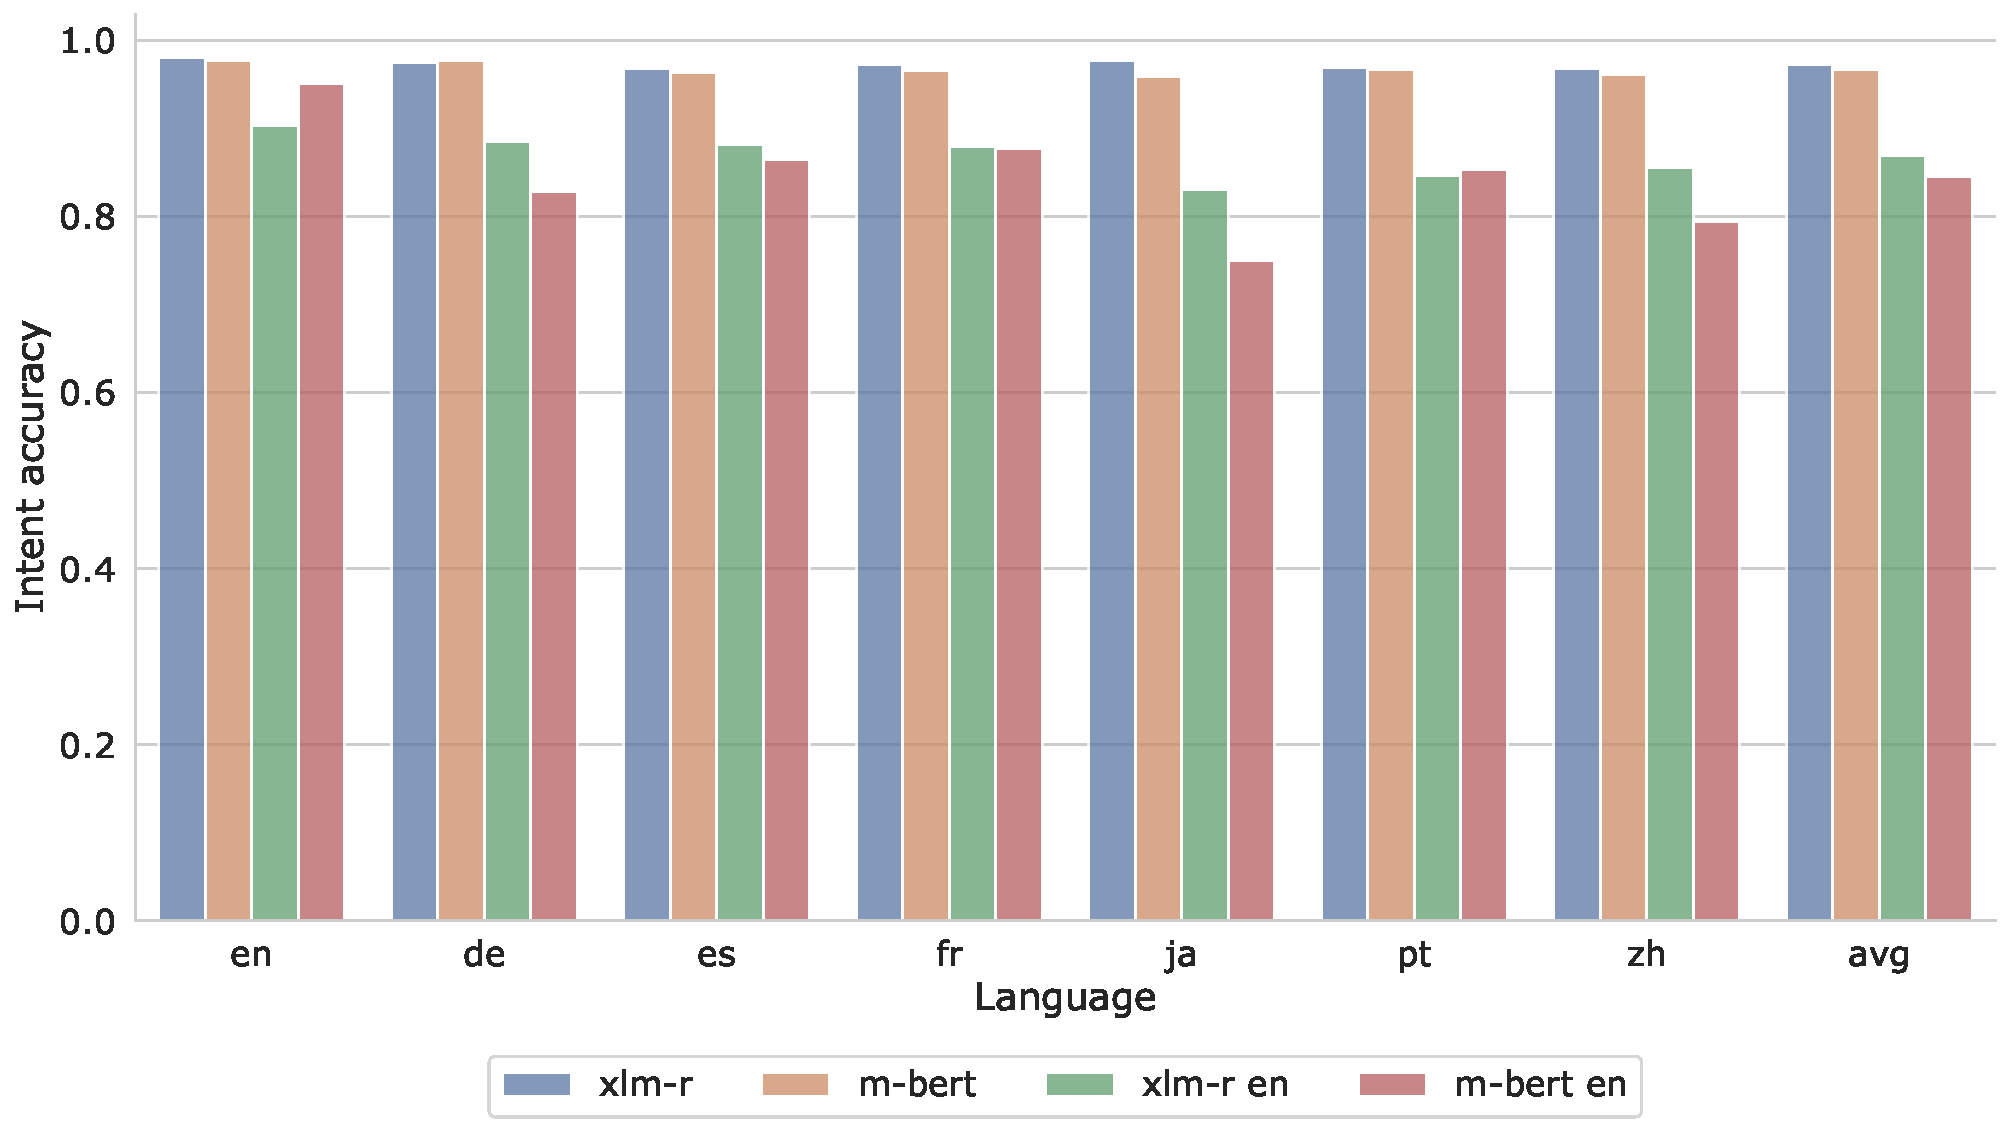
\includegraphics[width=\textwidth]{images/0}
    \caption{Сравнение моделей между собой \textbf{на тестовой выборке} датасета MultiAtis++ по метрике \textbf{Intent accuracy}.}\label{fig:figure0}
\end{figure}

Мы решили задачу классификации интентов и заполнения слотов.
На графике~\eqref{fig:figure0} можно увидеть сравнительную диаграмму для метрики Intent accuracy.
В данной секции с результатами мы будем приводить графики результатов только для этой метрики, графики двух других метрик и подробные таблицы с результатами можно найти в приложениях (графики в~\eqref{subsec:graphs}, таблицы в~\eqref{subsec:tables}).
\parВ своей работе мы обнаружили, что модель XLM-RoBERTa, обучавшаяся на всей тренировочной выборке имеет слегка лучшее качество, чем модель m-BERT\@.
Это объяснимо за счёт того, что XLM-RoBERTa обучалась на корпусе CommonCrawl, который на несколько порядков больше, чем аналогичный датасет для m-BERT\@.
Однако в целом обе модели показали примерно одинаковое качество и говорить о каких-то значительных различиях в данном контексте не приходится.
\parТак же мы обнаружили, что модели, обучавшиеся на английской тренировочной подвыборке имеют качество ощутимо хуже, чем их аналоги с полной выборки.
В дополнение к этому мы заметили, что модель XLM-RoBERTa показывает качество значительно хуже, чем m-BERT после обучения только на английском.
Это можно объяснить за счёт того, что данная языковая модель больше и требует большего количества данных для обучения.
Данное сравнение показывает, что перенос знаний ещё не в полной мере может соперничать с обучением модели на переведенных данных.

\subsubsection{Качество моделей после адверсариальных атак}

Мы провели две адверсариальные атаки на каждую из моделей и замерили качество.
Примеры атак на все модели можно найти в приложении~\eqref{subsec:examples}.
\parНа графике~\eqref{fig:figure3} можно увидеть сравнительную диаграмму после word-level атаки для метрики Intent accuracy.
На графике~\eqref{fig:figure6} можно увидеть сравнительную диаграмму после phrase-level атаки для метрики Intent accuracy.
\parВ своей работе мы обнаружили, что как и предполагалось качество после word-level атаки хуже, чем после phrase-level атаки.
Так же мы выяснили, что в целом модели XLM-RoBERTa и m-BERT достаточно хорошо справились с атаками и показали высокое качество.
\parВ своей работе мы убедились, что модель XLM-RoBERTa оказалось более робастной в данной задаче после адверсариальных атак, чем модель m-BERT\@.
Так же мы заметили, что модели, обученные на английской подвыборке гораздо хуже справлялись с атаками, нежели их аналоги, обученные на полной выборке.
Наиболее сильное влияние на качество оказывала атака с применением португальского языка, а так же китайского и японского.
Это объясняется низкоресурсностью португальского языка и иной морфологической структурой азиатских языков.
\parДополнительно мы заметили, что m-BERT обученный только на английской подвыборке гораздо лучше справляется с phrase-level атакой, однако хуже справляется с word-level атакой, чем XLM-RoBERTa.
Это объяснимо тем, что m-BERT обучается на Wikipedia, которая может в какой-то мере предоставить параллельные статьи на одну и ту же тему, таким образом у данной модели в обучающих данных присутствует некоторое выравнивание,
что позволило расположить языки соответствующим образом в признаковом пространстве.
Таким образом, m-BERT оказался более чувствителен к синтаксическим пертурбациям.
XLM-RoBERTa же обучалась на моноязычных данных, но гораздо большего объема, что привело к лучшему качеству после word-level атаки.

\begin{figure}[H]
    \centering
    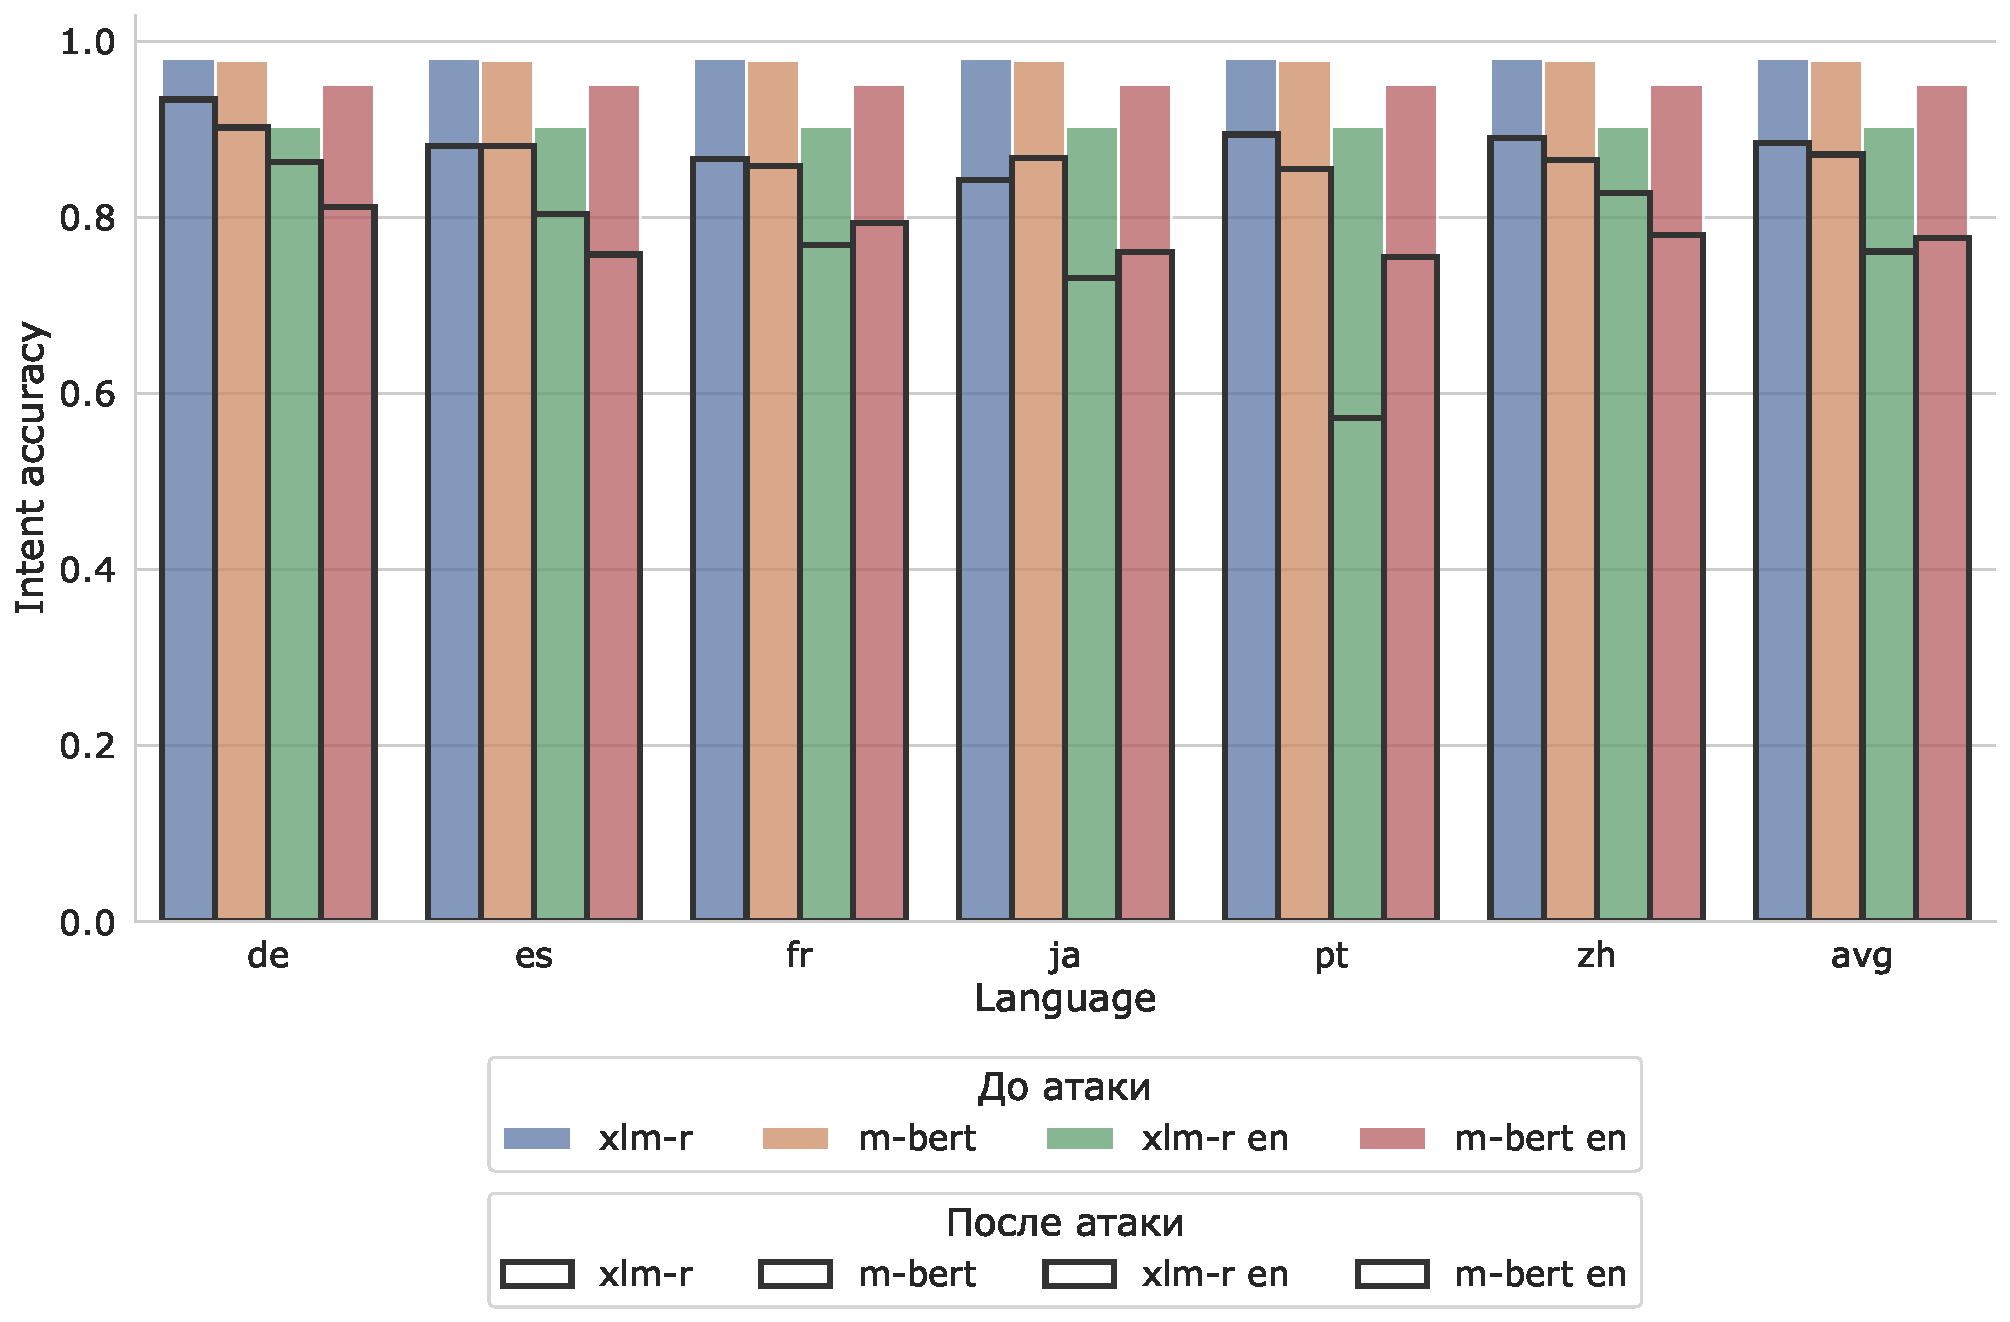
\includegraphics[width=\textwidth]{images/3}
    \caption{Сравнение моделей между собой после \textbf{word-level} атаки на тестовую выборку датасета MultiAtis++ по метрике \textbf{Intent accuracy}.}\label{fig:figure3}
\end{figure}

\begin{figure}[H]
    \centering
    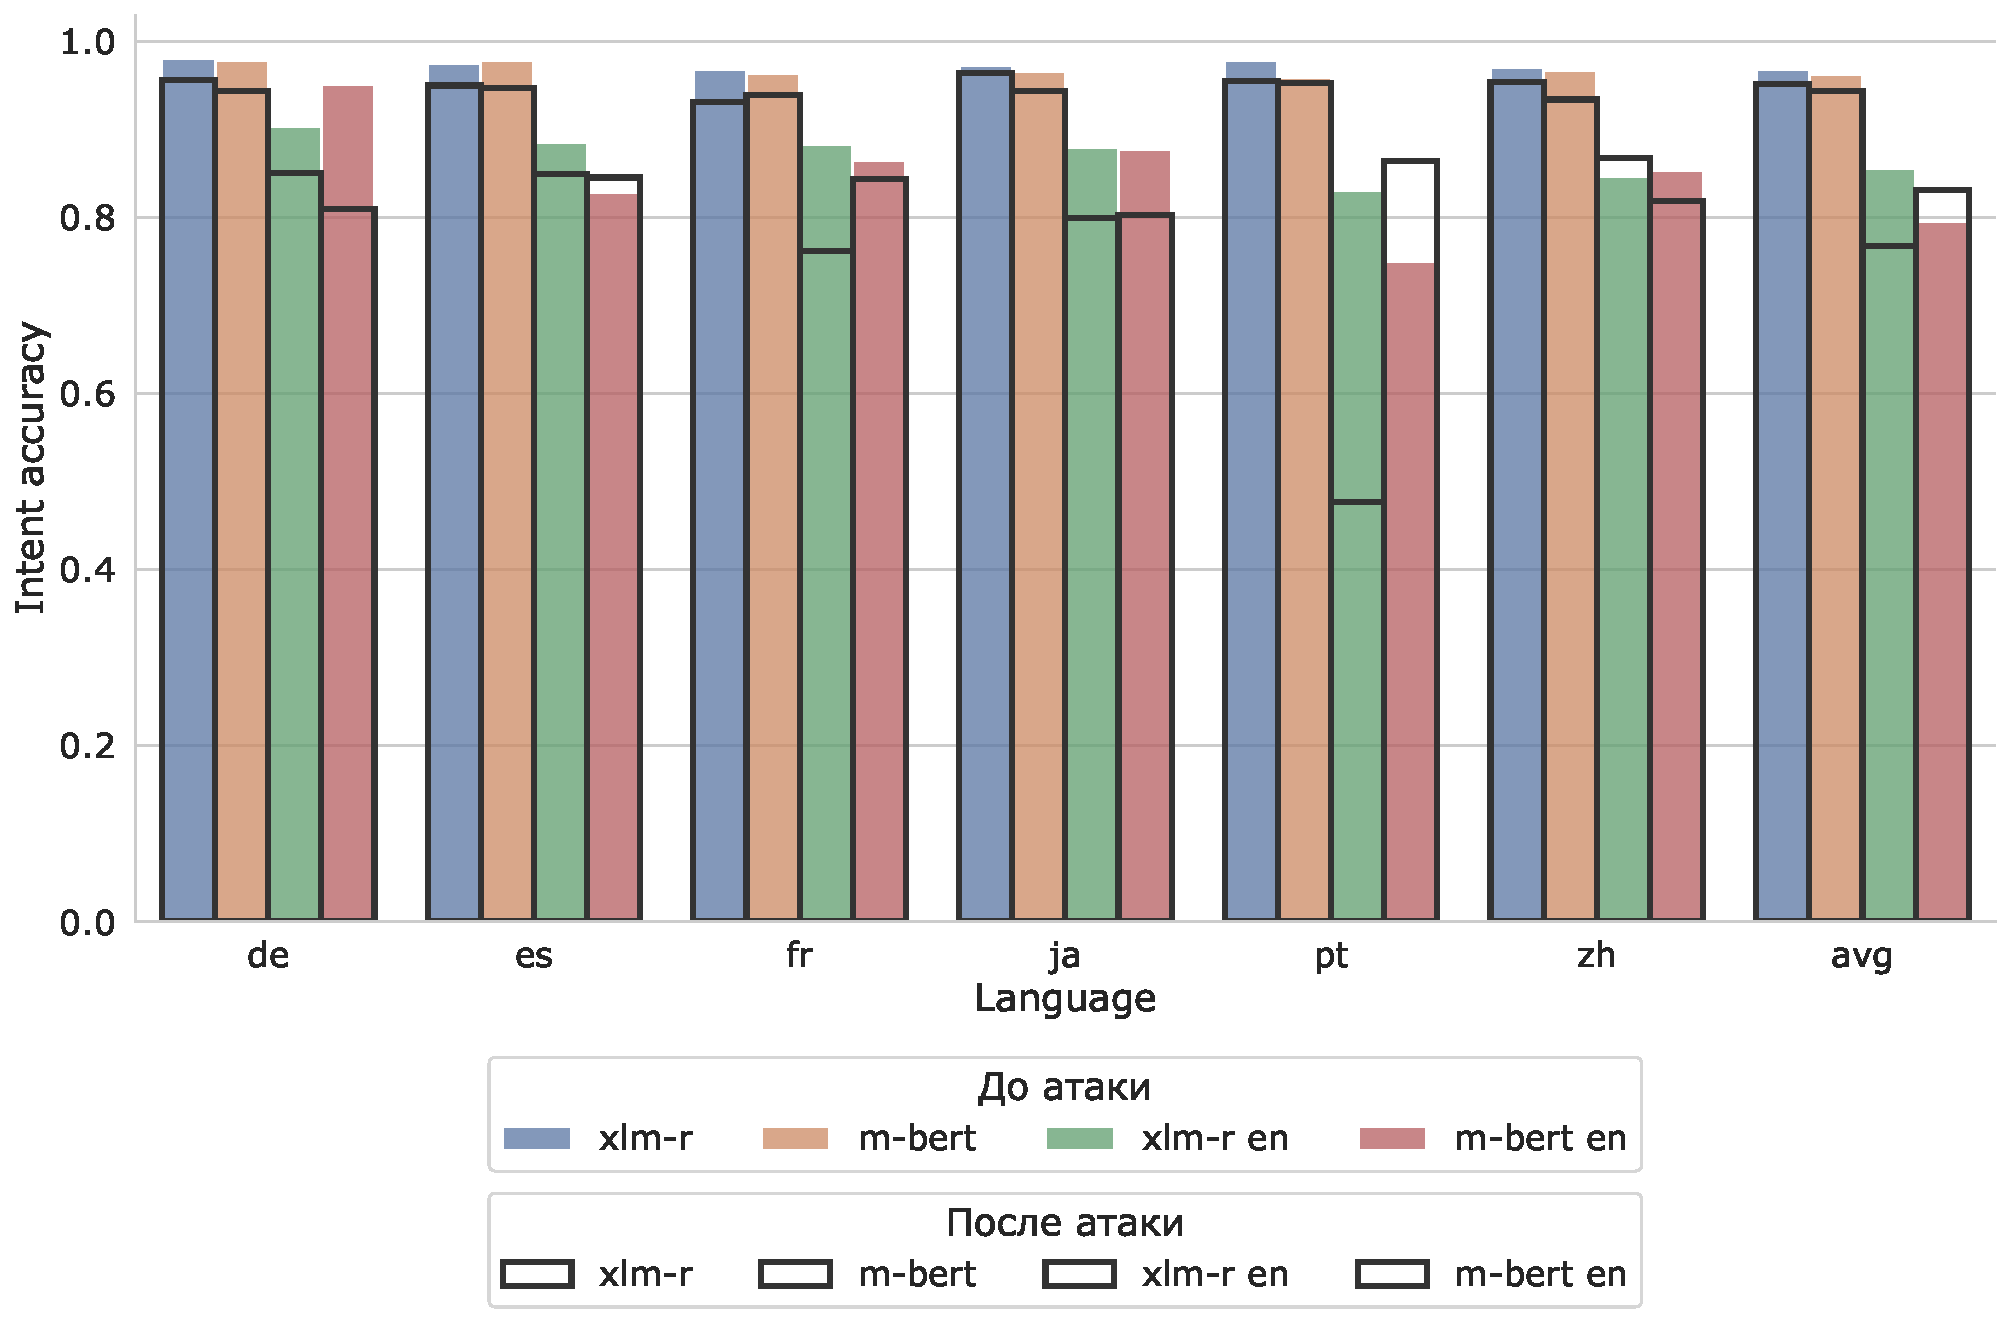
\includegraphics[width=\textwidth]{images/6}
    \caption{Сравнение моделей между собой после \textbf{phrase-level} атаки на тестовую выборку датасета MultiAtis++ по метрике \textbf{Intent accuracy}.}\label{fig:figure6}
\end{figure}

\begin{figure}[H]
    \centering
    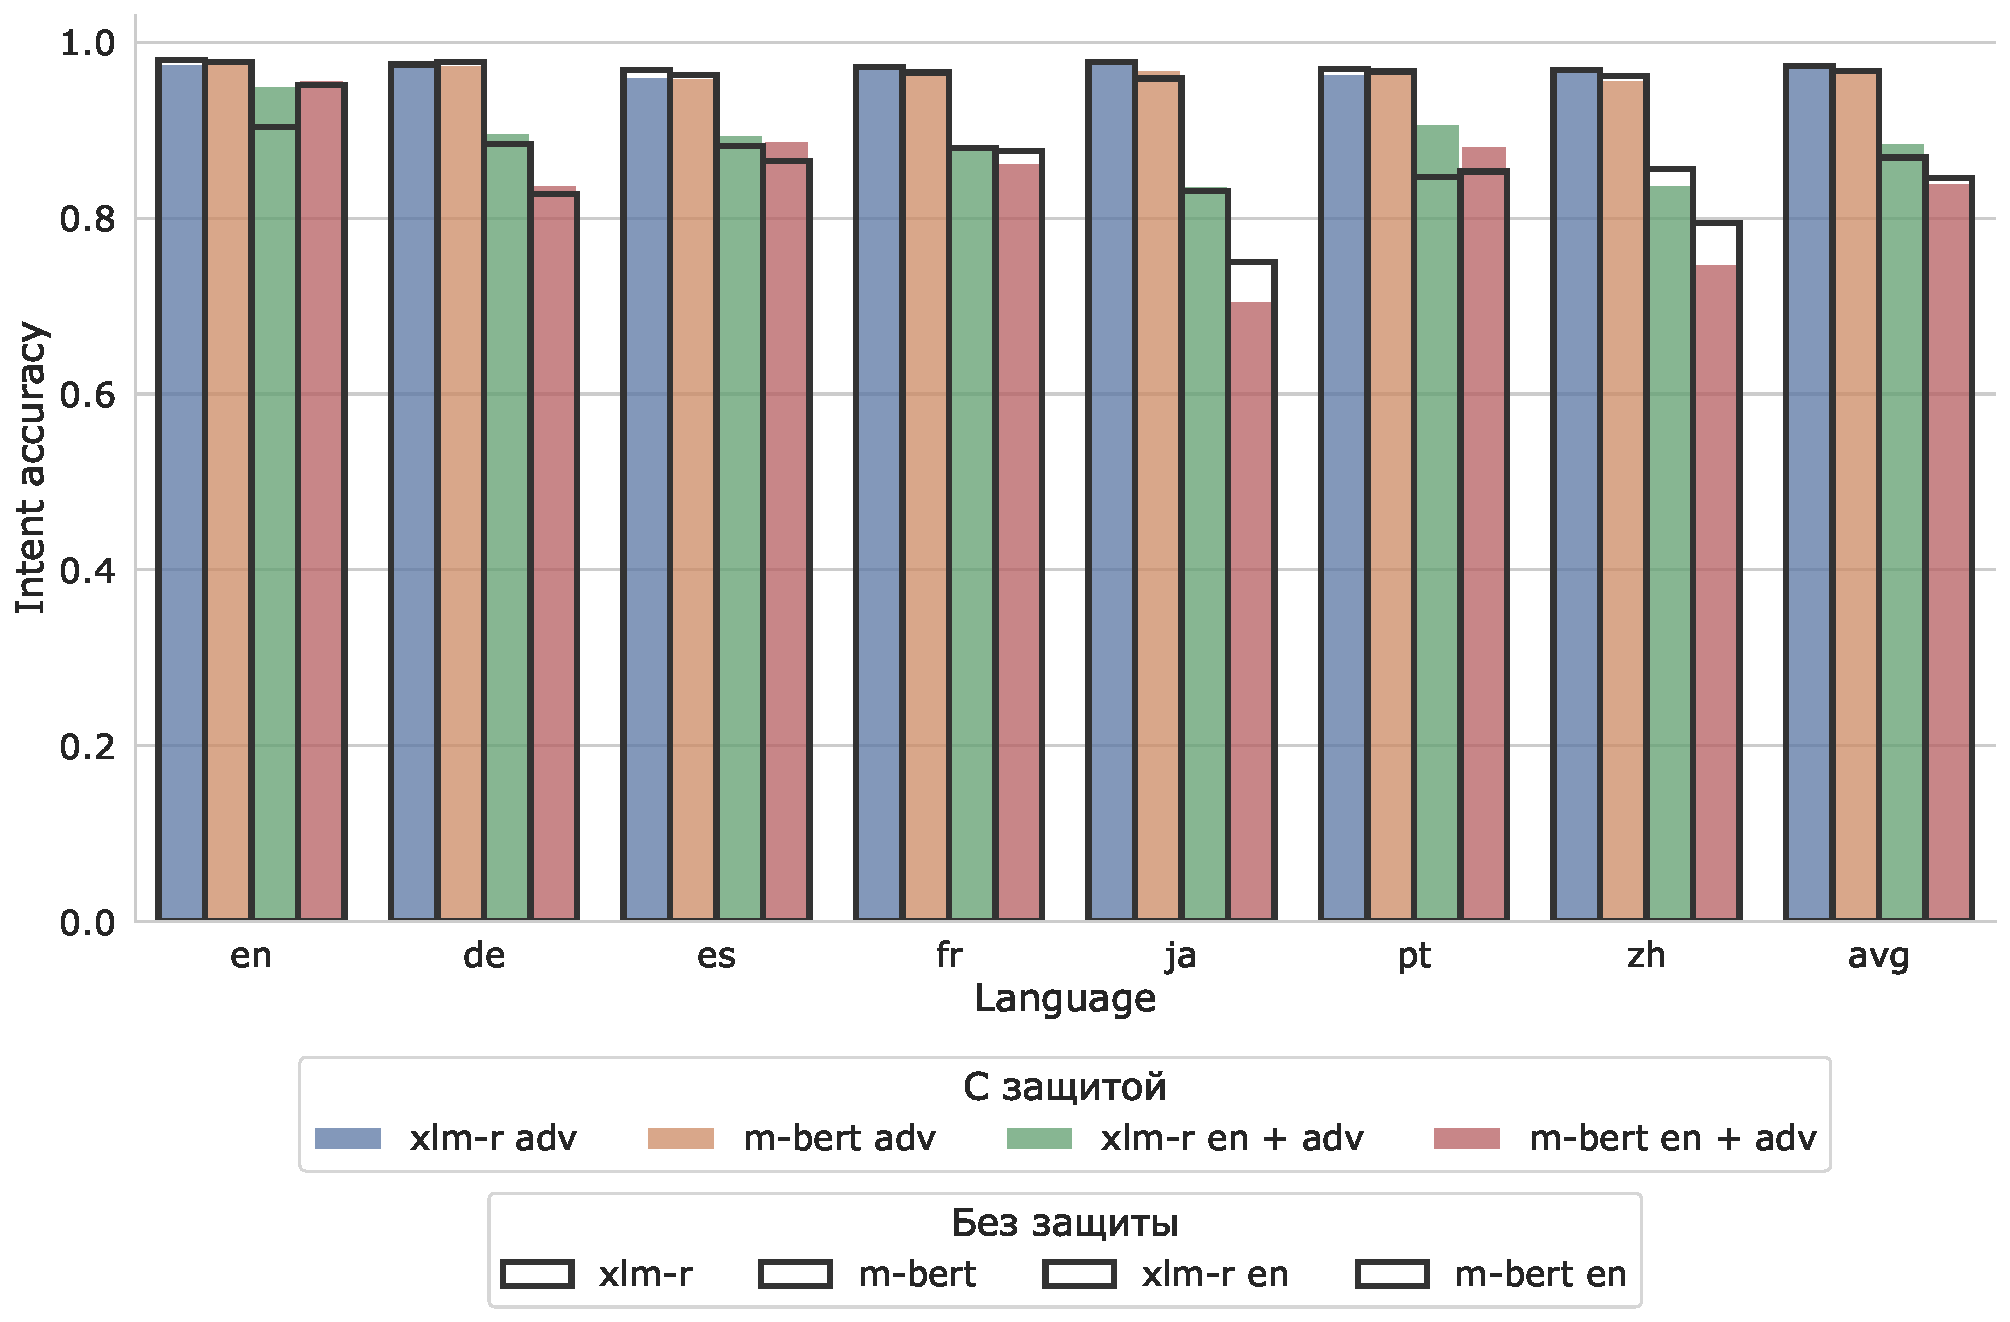
\includegraphics[width=\textwidth]{images/9}
    \caption{Сравнение моделей \textbf{с защитой} между собой \textbf{на тестовой выборке} датасета MultiAtis++ по метрике \textbf{Intent accuracy}.}\label{fig:figure9}
\end{figure}

\subsubsection{Влияние метода адверсариального предобучения}

Мы дообучили обе модели XLM-RoBERTa и m-BERT на нашей адверсариальной выборке в режиме маскированного моделирования языка.
На графике~\eqref{fig:figure9} можно видеть сравнительную диаграмму влияния метода защиты на качество моделей на тестовой выборке датасета MultiAtis++.
\parВ своей работе мы обнаружили, что дополнительная защита не повлияла на качество на тестовой выборке у моделей, обучаемых на полной тренировочной выборке.
В то же время модели обучаемые на английской подвыборке XLM-RoBERTa немного увеличила качество, а m-BERT уменьшил.
Это можно объяснить тем, что XLM-RoBERTa мы дали немного информации про отношения между языками, что позволило немного сместить взаиморасположение языков в признаковом пространстве.
В то же время эта же информация могла негативно повлиять на m-BERT с точки зрения выравниваний между языками.
\parНа графике~\eqref{fig:figure12} можно видеть сравнительную диаграмму влияния метода защиты на качество моделей после word-level атаки для метрики Intent accuracy.
На графике~\eqref{fig:figure15} можно видеть сравнительную диаграмму влияния метода защиты на качество моделей после phrase-level атаки для метрики Intent accuracy.
\parВо время исследования мы выяснили, что защита добавила качества после атак модели m-BERT, всем её вариациям.
Особенно подросло качество после word-level атаки, это можно объяснить тем, что мы внесли некоторый шум в распределение языков в пространстве признаков m-BERT и таким образом сделали его менее чувствительным к синтаксическим пертурбациям.
\parТак же мы выяснили, что защита негативно сказалась на качестве на азиатских языках после атаки, в большинстве своём качество упало для моделей с использованием защиты.
Это можно объяснить тем, что мы внесли некорректную информацию о взаиморасположении слов между собой в азиатских языках, что ухудшило качество и сделало модели более чувствительными к атакам.
\parВ своей работе мы заметили, что защита влияет наиболее сильно на модели, обученные на английской подвыборке, нежели на всей тренировочной выборке датасета.
Это можно объяснить тем, что модели, обучаемые на полной выборке, могут получить информацию об относительном расположении языков и в принципе обучиться для какого-то языка, в то время как другие модели такого сделать не могут.
\parВ целом защита больше повлияла на метрику Semantic accuracy, остальные две метрики изменяются в значительно меньшем соотношении.

\begin{figure}[H]
    \centering
    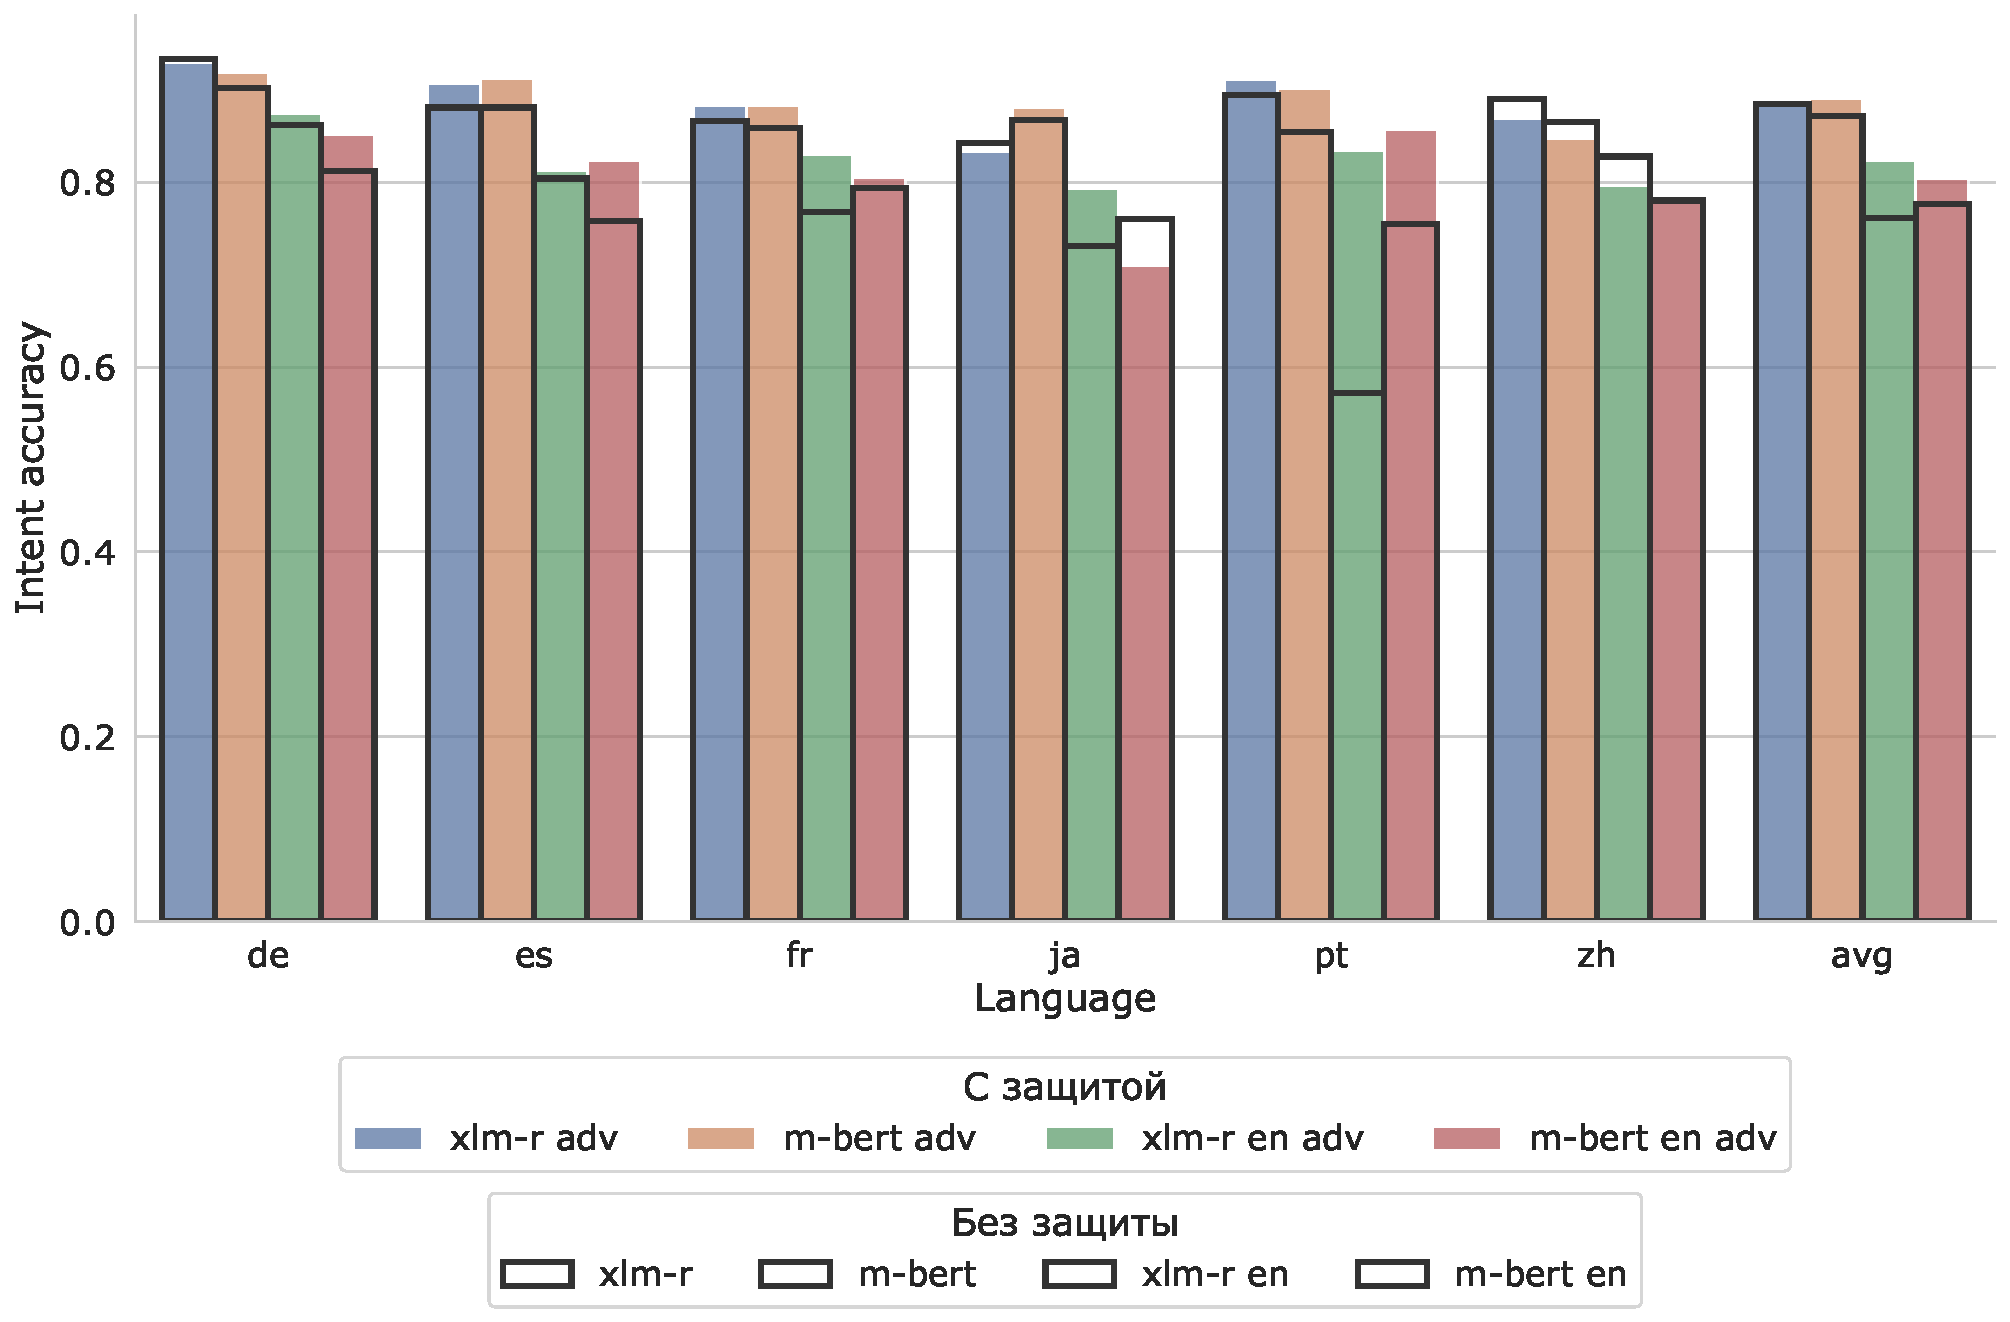
\includegraphics[width=\textwidth]{images/12}
    \caption{Сравнение моделей \textbf{с защитой} между собой после \textbf{word-level} атаки на тестовую выборку датасета MultiAtis++ по метрике \textbf{Intent accuracy}.}\label{fig:figure12}
\end{figure}

\parТак же хотелось бы сравнить между собой предложенный метод адверсариального предобучения и простое обучение на всей тренировочной выборке.
Можно рассматривать обучение на всех языках как своего рода защиту, которая повышает качество и позволяет моделям быть более устойчивыми к атакам и показывать в целом лучшее качество.
В своей работе мы получили результаты, которые позволяют сделать вывод, что если у нас есть обучающие данные для задачи заполнения слотов и классификации интентов на одном языке,
то будет лучше перевести эти данные на набор возможных языков и разметить, а затем обучить модель на всех таких данных.

\begin{figure}[H]
    \centering
    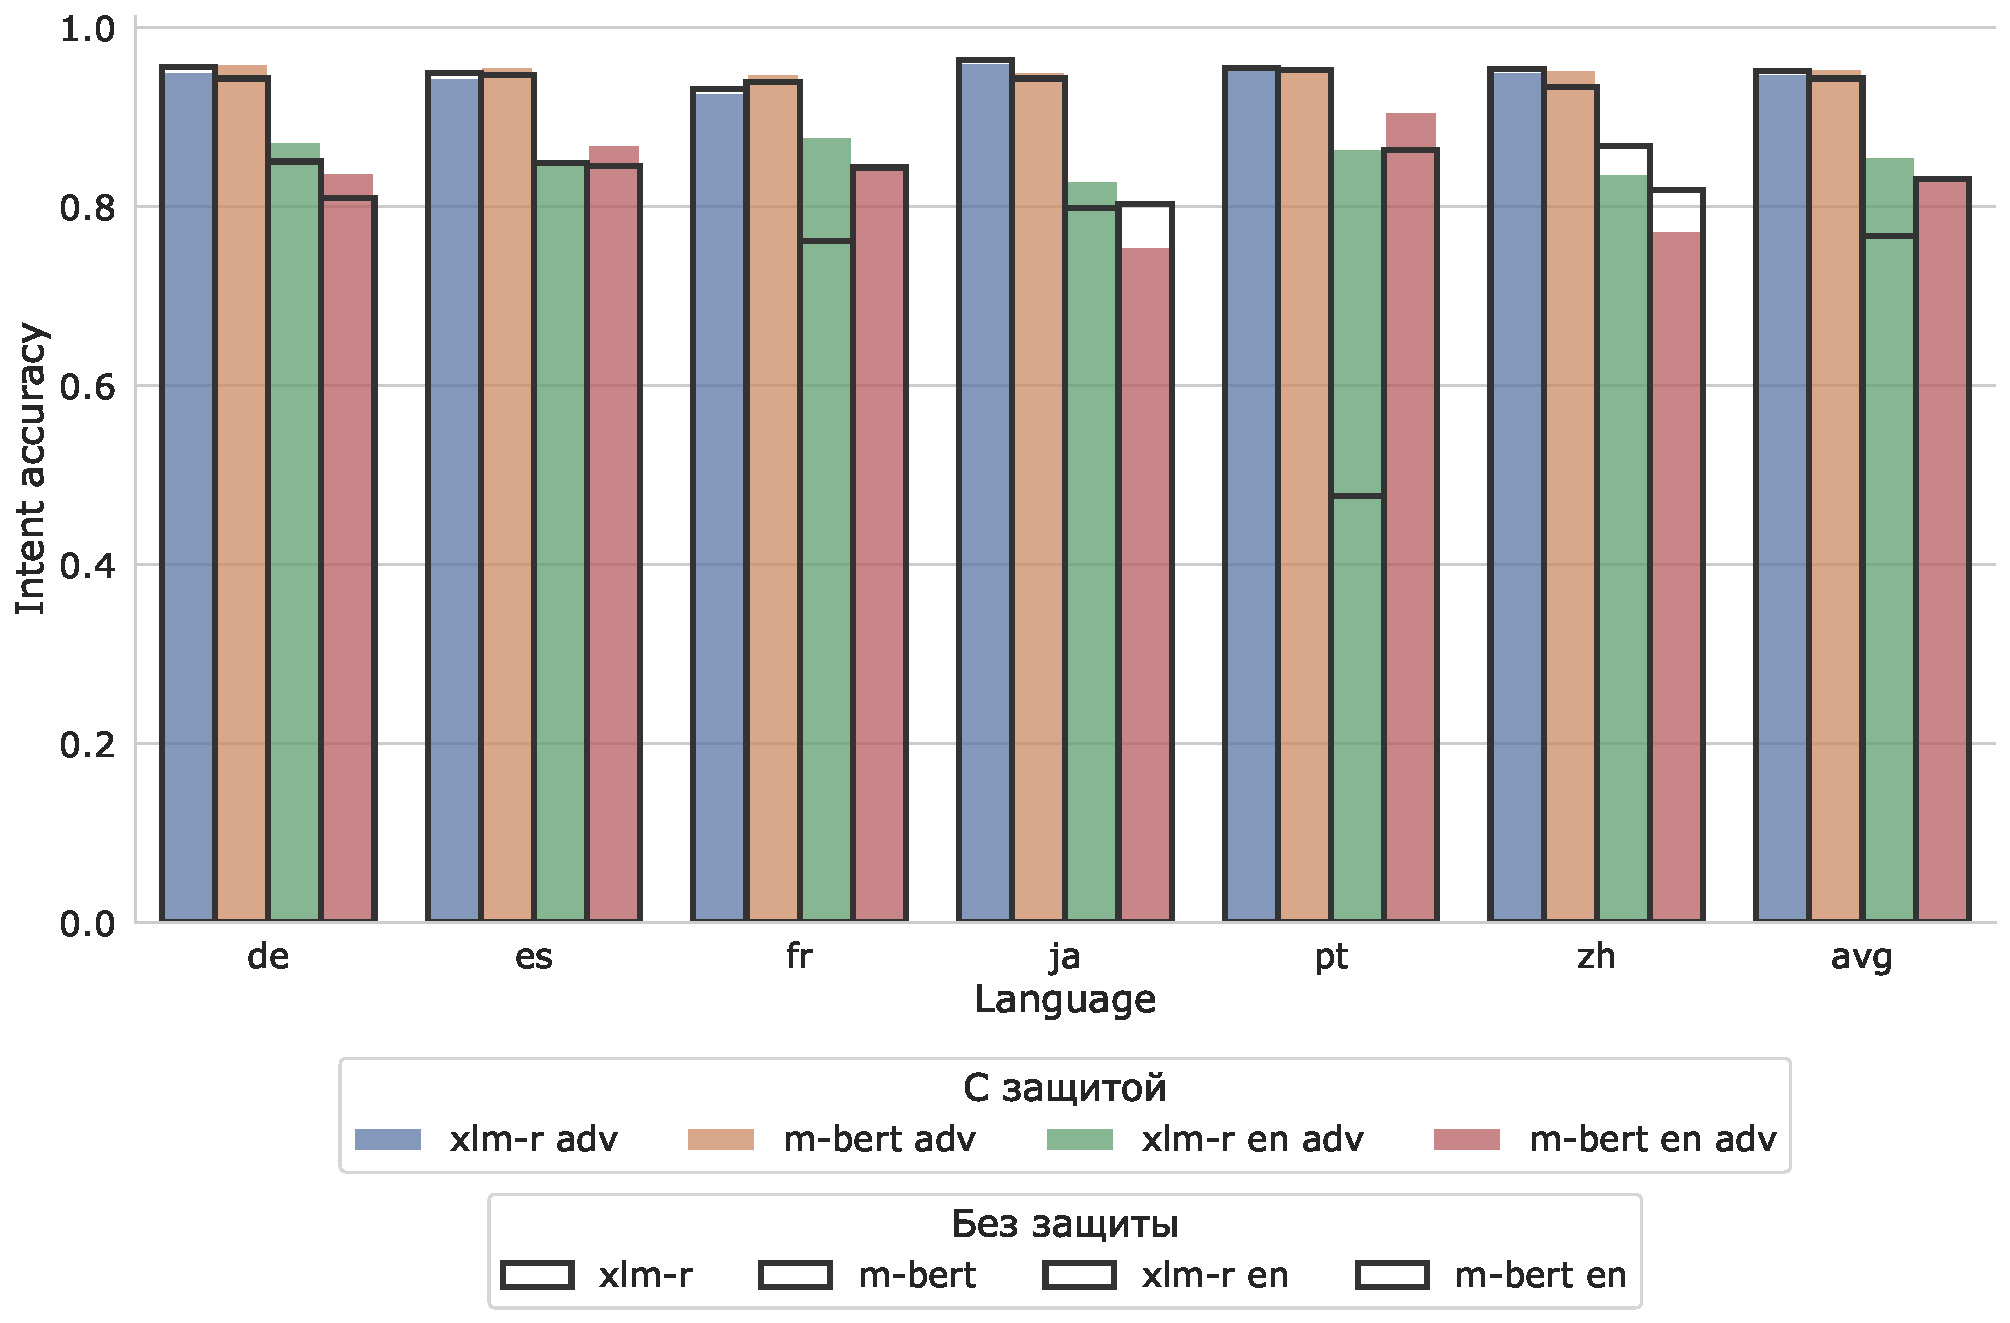
\includegraphics[width=\textwidth]{images/15}
    \caption{Сравнение моделей \textbf{с защитой} между собой после \textbf{phrase-level} атаки на тестовую выборку датасета MultiAtis++ по метрике \textbf{Intent accuracy}.}\label{fig:figure15}
\end{figure}
